\documentclass[12pt,a4paper]{article}
\usepackage[T1]{fontenc}
\usepackage[utf8]{inputenc}
\usepackage[brazil]{babel}
\usepackage{newtxtext,newtxmath,microtype,geometry,setspace,graphicx,booktabs}
\usepackage[colorlinks=true,citecolor=blue,urlcolor=blue,linkcolor=black]{hyperref}
\usepackage[alf]{abntex2cite}
\geometry{margin=2.5cm}
\setstretch{1.15}
\setlength{\parindent}{1.25cm}
\newcommand{\NRegistros}{8.424}
\newcommand{\NMeses}{312}
\newcommand{\NCelulas}{75.816}
\newcommand{\NAplicaveis}{46.656}
\newcommand{\NAusencias}{29.160}
\newcommand{\NLacunas}{0}
\newcommand{\NOcorrencias}{0}
\newcommand{\CIngenua}{61,54}
\newcommand{\CCondicionada}{100,00}

\title{Auditoria da completude temporal dos dados abertos de arrecadação federal por UF com Python}
\author{Giovanni Brígido\\
\small Receita Federal do Brasil --- Auditor-Fiscal\\
\small E-mail: \texttt{giovannibrigido@gmail.com}}
\date{}
\begin{document}
\maketitle
\begin{abstract}
Este estudo avalia a completude de dados públicos de arrecadação federal,
distinguindo lacunas de preenchimento de ausências previstas no dicionário de
dados. A prova de conceito aplica controles em Python à publicação por unidade
da Federação, no período de 2000 a 2025. O recorte contém \NRegistros{}
registros e cobre \NMeses{} meses nas 27 unidades federativas. Nove colunas
relativas à Cofins, ao PIS/Pasep e à CSLL foram avaliadas por intervalos de
publicação documentados. A contagem indiscriminada identificou \NAusencias{}
campos vazios; todos estavam fora dos intervalos de aplicabilidade definidos.
A completude passou de \CIngenua{}\% na medida indiscriminada para
\CCondicionada{}\% na medida condicionada. O resultado evidencia a importância
dos metadados na triagem de qualidade, sem certificar a exatidão dos montantes
arrecadados. O produto é um procedimento reproduzível de apoio à governança
da informação, acompanhado de regras, registros de execução e testes controlados.

\noindent\textbf{Palavras-chave:} qualidade de dados; arrecadação federal;
completude; governança; Python.
\end{abstract}

\section{Contextualização e descrição do problema}
A Receita Federal publica uma série de arrecadação mensal por unidade da
Federação, com valores em reais e categorias de receitas administradas e não
administradas pelo órgão \cite{rfbDados,rfbDicionario}. No contexto de uso desses
dados por um auditor, o problema aqui delimitado é avaliar se a série aberta
oferece cobertura adequada para análises e relatórios. Trata-se de uma
oportunidade de controle da informação, cuja relevância decorre da necessidade
de examinar completude e adequação dos dados antes de utilizá-los como evidência
\cite{gao2019}.

O dicionário registra mudanças na estrutura de publicação. Cofins, PIS/Pasep e
CSLL aparecem em colunas agregadas até dezembro de 2003 e em categorias
``Financeiras'' e ``Demais'' a partir de janeiro de 2004
\cite{rfbDicionario}. Assim, a ausência de um valor pode decorrer da estrutura
histórica do arquivo. A questão de pesquisa é: \textit{como incorporar os
intervalos documentados de publicação para evitar que ausências previstas
sejam indevidamente encaminhadas como falhas de completude?}

A proposta busca reduzir revisões desnecessárias e preservar o significado
dos campos, coerentemente com a compreensão de que qualidade depende do
contexto de uso \cite{wang1996}. Não se afirma que a Receita utilize hoje uma
validação indiscriminada: essa abordagem foi construída como referência de
comparação. Tampouco o estudo identifica contribuintes, estima sonegação ou
atribui desempenho a unidades administrativas.

\section{Fundamentação e técnica selecionada}
A técnica escolhida é a verificação de qualidade por regras determinísticas,
com cruzamento entre observações e metadados temporais. A literatura distingue
qualidade de mera precisão e reconhece dimensões contextuais e de representação
\cite{wang1996}. A orientação do GAO também relaciona a confiabilidade dos
dados à finalidade da auditoria \cite{gao2019}. Neste estudo, operacionaliza-se
a completude como preenchimento das células para as quais o dicionário prevê
a publicação da categoria correspondente.

Seja $A_{ij}=1$ quando a coluna $j$ é aplicável ao mês do registro $i$, e
$P_{ij}=1$ quando existe conteúdo não vazio. As duas medidas são:
\[
C_{\mathrm{simples}}=\frac{\sum_{i,j}P_{ij}}{N},\qquad
C_{\mathrm{temporal}}=\frac{\sum_{i,j}A_{ij}P_{ij}}{\sum_{i,j}A_{ij}}.
\]
O denominador $N$ corresponde às células das nove colunas no recorte. O conteúdo
``0'' conta como preenchido. A validade numérica é examinada separadamente.
Presença fora do intervalo gera uma ocorrência própria, pois pode indicar
mudança do arquivo ou desatualização do dicionário.

A abordagem é apropriada porque cada decisão pode ser explicada por uma regra
e uma data verificáveis. Um modelo de linguagem acrescentaria incerteza à
aplicação de intervalos já explícitos. O registro das regras e dos indicadores
adota o princípio de explicitar as métricas e sua proveniência, discutido pelo
W3C \cite{w3c2016}; não houve implementação do vocabulário RDF dessa organização.

\section{Metodologia e dados}
Foram baixados diretamente do repositório oficial o CSV e seu dicionário em PDF,
com preservação dos arquivos originais, endereços, horário UTC e hashes SHA-256.
A análise utiliza janeiro de 2000 a dezembro de 2025, mantendo um intervalo de
anos completos. O arquivo adquirido também contém meses de 2026, que ficaram
fora do recorte. A rotina verifica os hashes antes de analisar e reutiliza a
cópia congelada em execuções posteriores.

O fluxo em Python compreendeu: aquisição com \texttt{requests}; leitura como
texto com \texttt{pandas}, separador ponto e vírgula e codificação Latin-1;
validação de datas, UFs e chave composta ano--mês--UF; comparação com o produto
cartesiano de meses e 27 UFs; validação lexical das colunas de valores;
cruzamento das nove colunas com regras em JSON; e exportação de tabelas e
figura com \texttt{matplotlib}. O dicionário é a fonte dos intervalos, transcritos
antes da comparação com os campos vazios \cite{rfbDicionario}.

Cada célula do recorte recebeu um de quatro estados: preenchida e aplicável;
ausente e aplicável; ausente fora do intervalo; ou preenchida fora do intervalo.
Os dois estados que divergem da expectativa documental são encaminhados para
revisão. As demais 33 colunas de valores receberam apenas a checagem lexical;
sua completude temporal não foi avaliada. Não houve soma indiscriminada de
categorias nem preenchimento automático de vazios com zero.

O arquivo apresenta diferentes convenções de separadores numéricos. O controle
reconhece sintaxes com vírgula ou ponto como separador decimal e agrupamentos
de milhar compatíveis, mas preserva o texto original. Uma representação
ambígua não é convertida automaticamente. Consequentemente, o estudo verifica
presença e formato, sem recalcular valores ou certificar sua exatidão.

A validação funcional introduziu defeitos isolados em cópias da base:
ausência aplicável, presença fora do intervalo, texto não numérico, mês ou UF
inválidos, duplicação e remoção de registro. Casos de controle verificaram
zero, sinal negativo, separadores e os meses adjacentes à mudança de 2004.
Os resultados foram comparados com as classes esperadas. Esse procedimento
testa a implementação e não estima precisão ou revocação em falhas reais,
que exigiriam avaliação independente.

Os arquivos analisados são agregados por UF e mês, sem identificadores de
pessoas ou empresas. O processamento não consulta bases sigilosas nem transmite
dados a serviços de IA. Uma adoção institucional dependeria da validação das
regras pelo responsável pela publicação e da atribuição de responsabilidades
para manter metadados e tratar ocorrências, em linha com a participação dos
envolvidos na avaliação de confiabilidade \cite{gao2019}.

\section{Resultados e impacto na governança}
O recorte apresentou \NRegistros{} registros, equivalentes a \NMeses{} meses
vezes 27 UFs, sem chaves duplicadas ou ausentes. Não foram detectados meses ou
UFs inválidos nem representações numéricas fora das sintaxes aceitas. Para as
nove colunas, foram classificadas \NCelulas{} células, das quais
\NAplicaveis{} pertenciam aos intervalos documentados.

\begin{table}[htbp]
\centering
\caption{Completude das nove colunas no período de 2000--2025.}
\small
\begin{tabular}{lr}
\toprule Indicador & Resultado\\\midrule
Células avaliadas & \NCelulas{}\\
Células aplicáveis & \NAplicaveis{}\\
Vazios identificados sem regra temporal & \NAusencias{}\\
Ausências dentro do intervalo aplicável & \NLacunas{}\\
Completude sem regra temporal & \CIngenua{}\%\\
Completude condicionada ao intervalo & \CCondicionada{}\%\\
\bottomrule
\end{tabular}
\label{tab:resultados}
\end{table}

Todas as \NAusencias{} ausências foram classificadas como previstas, sem
presenças fora do intervalo. A mudança entre as medidas resulta da alteração
do denominador, e não de correção da base. A figura mostra como a multiplicação
das categorias publicadas em 2004 altera a contagem simples. A completude
condicionada permanece em 100\% nas nove colunas, resultado restrito à definição
adotada e à versão do arquivo.

\begin{figure}[htbp]
\centering
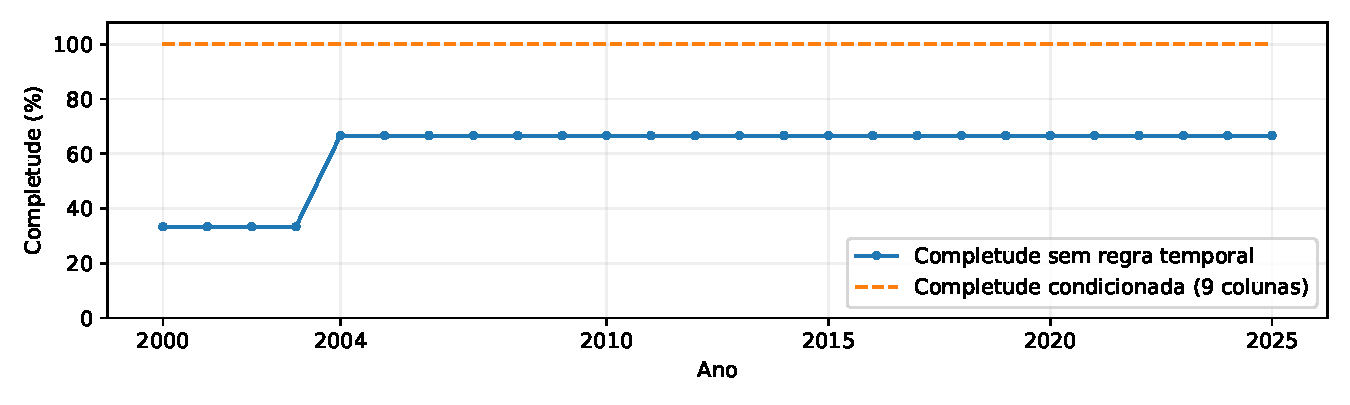
\includegraphics[width=\linewidth]{figuras/completude.pdf}
\caption{Comparação anual das medidas nas nove colunas selecionadas.}
\end{figure}

Os 13 cenários controlados passaram pelos critérios esperados. O produto
operacional é uma tabela de ocorrências com chave, coluna, regra e valor
original, acompanhada da classificação de todas as células do recorte. Na base
observada, a tabela ficou sem ocorrências segundo os controles definidos. Um
uso possível é verificar novas versões antes de incorporá-las a relatórios e
encaminhar divergências ao responsável pelos dados.

Os ganhos de tempo e de redução de retrabalho permanecem potenciais, pois não
foram medidos com usuários. O estudo não compara a arrecadação publicada com
documentos de origem e não avalia pontualidade das divulgações. Regras
desatualizadas podem produzir alertas indevidos; valores incorretos, mas
preenchidos e sintaticamente válidos, podem passar despercebidos. Uma métrica
favorável em um aspecto não resolve a avaliação de adequação global dos dados
\cite{wang1996,w3c2016}.

\section{Considerações finais}
A prova de conceito demonstrou que metadados temporais modificam
substancialmente a interpretação da completude no recorte estudado. Sua
contribuição é um controle simples, explicável e reproduzível para a governança
dos dados públicos de arrecadação. Os resultados permitem separar ausências
documentadas de exceções que requerem investigação, sem transformar completude
em garantia de exatidão. Como próximos passos, propõe-se validar as regras com
o responsável pela base, ampliar a cobertura temporal das demais categorias e
testar o procedimento em novas versões, preservando histórico de mudanças e
medindo o esforço de revisão.

\clearpage
\bibliographystyle{abntex2-alf}
\begingroup\small\setstretch{1.0}
\bibliography{referencias}
\endgroup
\end{document}
